\documentclass[tikz,border=2pt,11pt]{standalone}
\usetikzlibrary{arrows.meta}
\usetikzlibrary{positioning}
\usepackage{amsmath}
\usepackage{amssymb}
\usepackage{tikz}
\newcommand{\doi}[1]{\href{https://doi.org/#1}{\nolinkurl{doi:#1}}}
\newcommand{\R}{\mathbb R}
\newcommand{\Z}{\mathbb Z}
\newcommand{\N}{\mathbb N}
\newcommand{\C}{\mathbb C}
\newcommand{\T}{\mathbb T}
\newcommand{\ind}{\mathbf 1}
\DeclareMathOperator{\diag}{diag}
\DeclareMathOperator{\ran}{ran}
\begin{document}
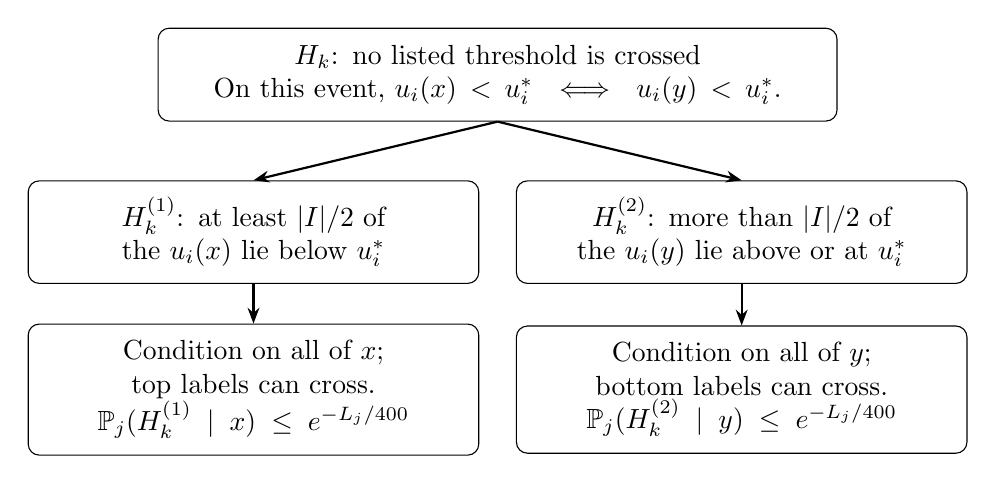
\begin{tikzpicture}[
  box/.style={draw,rounded corners,align=center,text width=5.3cm,
              minimum height=1.1cm,inner sep=6pt},
  arr/.style={-{Stealth[length=2mm]},thick}]
\node[box,text width=8.2cm] (b) at (0,0)
 {$H_k$: no listed threshold is crossed\\
  On this event, $u_i(x)<u_i^*\iff u_i(y)<u_i^*$.};
\node[box] (x) at (-3.1,-2)
 {$H_k^{(1)}$: at least $|I|/2$ of the $u_i(x)$ lie below $u_i^*$};
\node[box] (y) at (3.1,-2)
 {$H_k^{(2)}$: more than $|I|/2$ of the $u_i(y)$ lie above or at $u_i^*$};
\node[box] (cx) at (-3.1,-4)
 {Condition on all of $x$;\\
  top labels can cross.\\
  $\mathbb P_j(H_k^{(1)}\mid x)\le e^{-L_j/400}$};
\node[box] (cy) at (3.1,-4)
 {Condition on all of $y$;\\
  bottom labels can cross.\\
  $\mathbb P_j(H_k^{(2)}\mid y)\le e^{-L_j/400}$};
\draw[arr] (b.south) -- (x.north);
\draw[arr] (b.south) -- (y.north);
\draw[arr] (x) -- (cx);
\draw[arr] (y) -- (cy);
\end{tikzpicture}
\end{document}
